\documentclass[]{politex}

% ========== Packages ==========
\usepackage[utf8]{inputenc}
\usepackage{amsmath,amsthm,amsfonts,amssymb}
\usepackage{graphicx,cite,enumerate}
\usepackage{subfiles}
\usepackage{caption}
\usepackage{pdfpages}
\usepackage{adjustbox}
\usepackage{wrapfig,lipsum}
\usepackage{verbatim}
\usepackage{listings}
\usepackage{array}

% ========== Language options ==========
\usepackage[brazil]{babel}

% ========== ABNT (requer ABNTeX 2) ==========
%	http://www.ctan.org/tex-archive/macros/latex/contrib/abntex2
\usepackage[num]{abntex2cite}

% ========== Lorem ipsum ==========
\usepackage{blindtext}

% ========== Opções do documento ==========
% Título
\titulo{Desenvolvimento de Equipamentos para Hospital Universitário da USP}

% Autor
\autor{Thomaz Akira Furukawa}

% Orientador / Coorientador
\orientador{Leopoldo Rideki Yoshioka}
\coorientador{Oswaldo Horikawa}

% Tipo de documento
\tcc{}
%\dissertacao{Engenharia Elétrica}
%\teseDOC{Engenharia Elétrica}
%\teseLD
%\memorialLD

% Departamento e área de concentração
\departamento{Engenharia de Sistemas Eletrônicos}
\areaConcentracao{Engenharia Mecatrônica}

% Local
\local{São Paulo}

% Ano
\data{2022}

\begin{document}
% ========== Capa e folhas de rosto ==========
\capa
\falsafolhaderosto
\folhaderosto

%========== Folha de assinaturas (opcional) ==========
%\begin{folhadeaprovacao}
	\assinatura{Prof. Dr. Leopoldo Rideki Yoshioka}
	\assinatura{Prof. Dr. Oswaldo Horikawa}
%	\assinatura{Prof.\ Y}
%	\assinatura{Prof.\ Z}
%\end{folhadeaprovacao}

% ========== Ficha catalográfica ==========
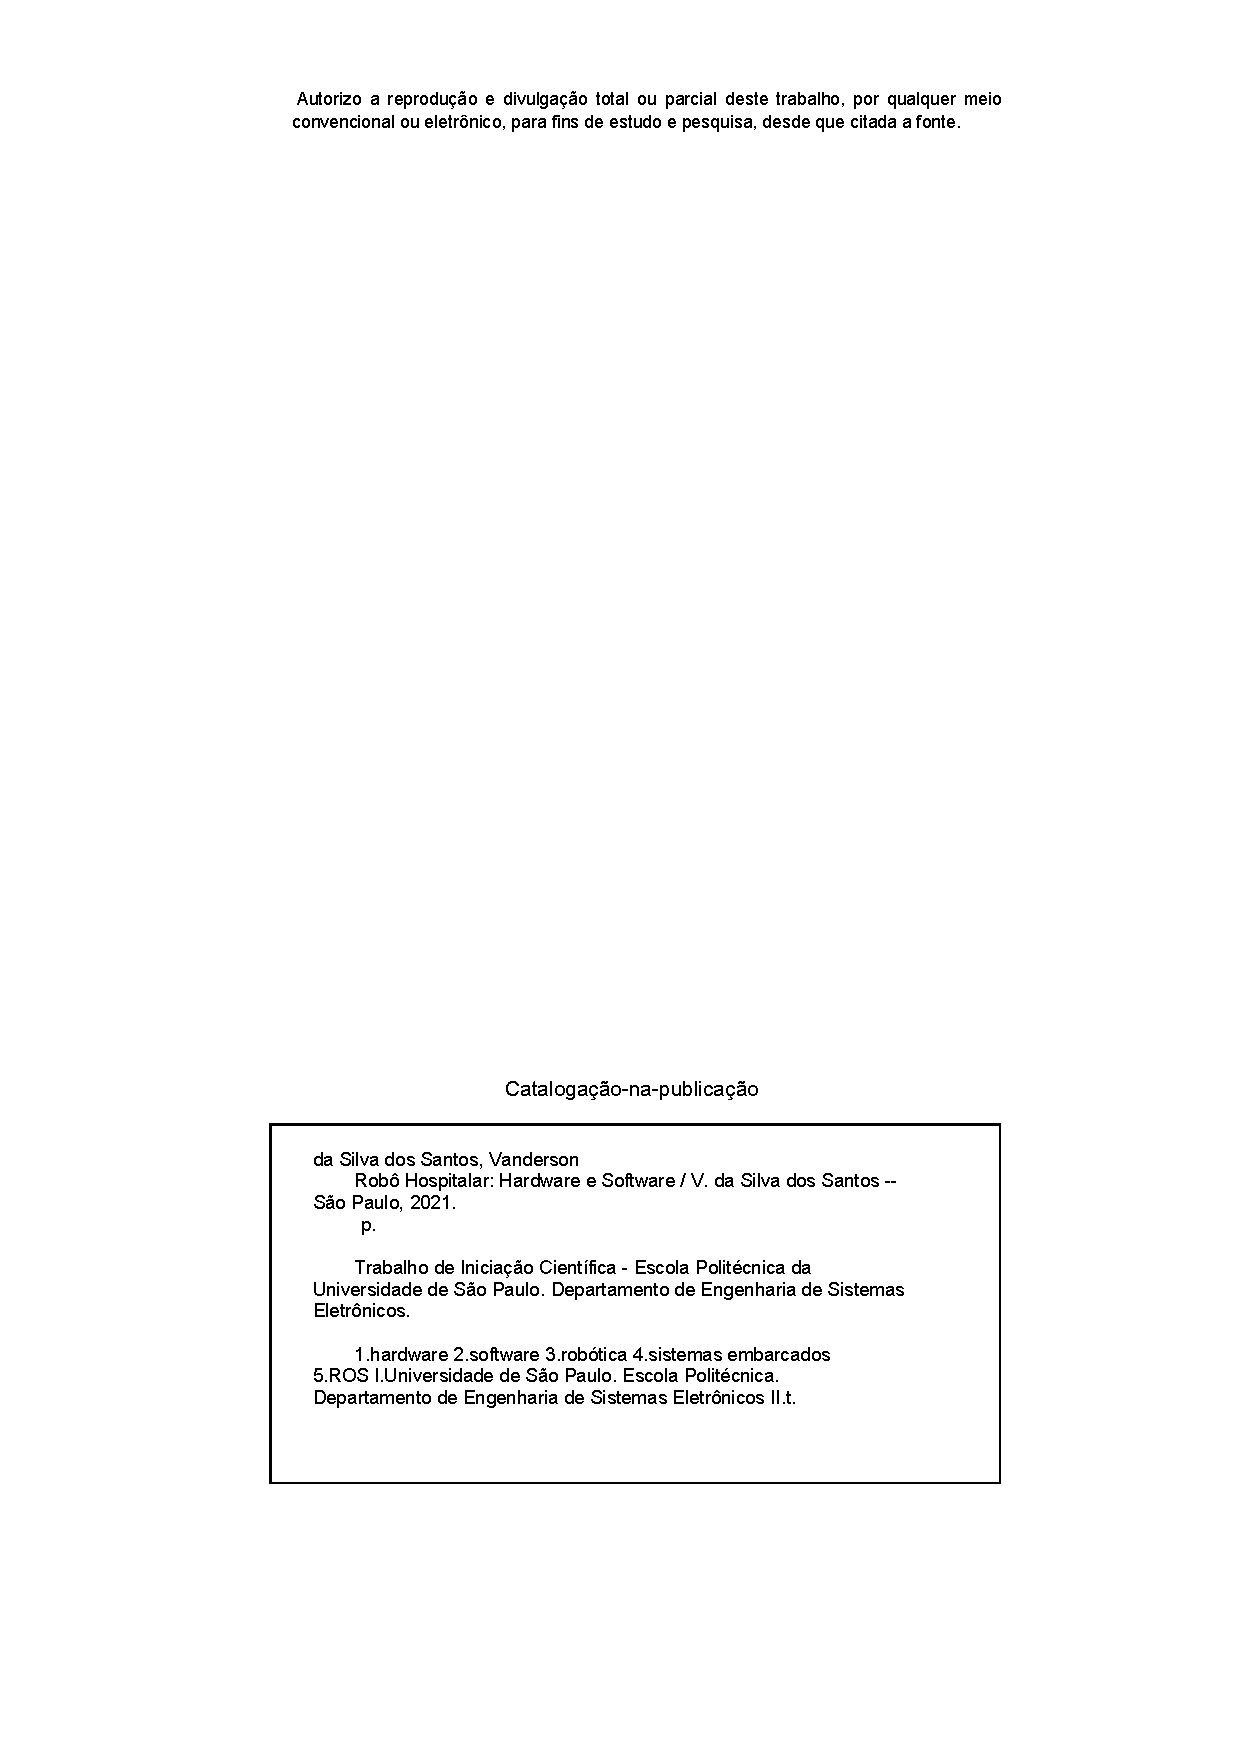
\includepdf{ficha_catalografica.pdf}

% ========== Dedicatória (opcional) ==========
\dedicatoria{Dedico esse trabalho aos atuais e futuros integrantes da ZIMA - Soluções Medico Hospitalares}

% ========== Agradecimentos ==========
\begin{agradecimentos}

Primeiramente, à minha família, que me forneceram inspiração, suporte emocional e financeiro para que eu chegasse até a universidade.

Ao meus professores orientadores, Leopoldo Yoshioka, pela a oportunidade de participar do grupo , fazer a manutenção do projeto e sempre dar suporte, tanto em ajuda, quanto em ensinamentos através de boas conversas e alguma risadas. Ao Professor Oswaldo Horikawa, que foi um forte auxílio técnico no desenvolvimento dos projetos e me inspirou a ser um engenheiro melhor.

Aos coordenadores de área e antigos membros, Vanderson Santos, Lucas Boccia, Lucas Grob, Wu Kam Long, Pedro Croso, Caio Oliveria, Lucas Junji e Joao Magano que sem essa equipe nada do que será apresentado seria possível.


\end{agradecimentos}

% ========== Epígrafe (opcional) ==========
\epigrafe{%
	\emph{``Para ganhar, tem que jogar bem e dar sorte.''}
	\begin{flushright}
		- Josué Ramalho da Silva
	\end{flushright}
}

% ========== Resumo ==========
\begin{resumo}
Desde 2020, a Escola Politécnica e Hospital Universitário da USP colaboram juntos para o desenvolvimento de soluções tecnológicas na área da saúde. O trabalho de incentivo a inovação foi o responsável pelo projeto Robô Hospitalar, robô autônomo para entregas de exames laboratorias, que chamou atenção dos colaboradores do Hospital para as oportunidades de inserir a tecnologia para inovar na saúde. Com o desenvolvimento do projeto e a entrega de resutados concretos, novas oportunidades surgiram, sendo duas delas sementes de dois novos projetos: o Dispensador de Remédios da Farmácia do HU e o aparelho de reabilitação Ciclo Ergômetro. Com a aproximação da Escola Politécnica e o Hospital Universitário da USP o incentivo a inovação se deu de diversas maneiras, não se limitando a entrega de projetos mas também a criação de grupos focados em inovação na saúde.
%
\\[3\baselineskip]
%
\textbf{Palavras-Chave} -- Automação, Algoritmos de Controle, Programação de Embarcados, Robótica, Saúde, Eletromédicos, Hospitalar, Inovação.
\end{resumo}

\begin{comment}

% ========== Abstract ==========
\begin{abstract}
Abstract...
%
\\[3\baselineskip]
%
\textbf{Keywords} -- Word, Word, Word, Word, Word.
\end{abstract}
\end{comment}
% ========== Listas (opcional) ==========
\listadefiguras
\listadetabelas

% ========== Sumário ==========
\sumario

% ========== Elementos textuais ==========

% ========== Parte 1: Introdução ==========
\part{Introdução}
\subfile{chapters/introducao} % em qual contexto foi possivel realizar a construção das maquinas e a criação da zima

\subfile{chapters/objetivo} % objetivo golgi ciclo robo e zima

\subfile{chapters/motivacao} % motivação

\subfile{chapters/metodologia} % como foi a concepção e fabricação

\subfile{chapters/arquitetura_do_projeto} % como a equipe se organizou e qual é a arquitetura de cada um

% ========== Parte 2: Hardware ==========
\part{Hardware} 

\subfile{chapters/distribuicao_de_energia}

\subfile{chapters/modulos_embarcados}

% ========== Parte 3: Software ==========
\part{Software}

\subfile{chapters/ambiente_de_simulacao}

\subfile{chapters/algoritmos_de_controle}

\subfile{chapters/integracao_software_hardware}

\begin{comment} % se sobrar tempo comentar


\subfile{chapters/desenvolvimento_web_mobile}
\end{comment}

% ========== Parte 4: Software ==========
\part{Resultados}

No âmbito da computação e da eletrônica, o software e hardware, que andam muito próximos um do outro, os resultados foram satisfatórios, mas nada além disso. Foi bastante trabalho em pouco tempo, porém, não foram realizados tantos testes quanto foi idealizado por conta de períodos sem poder frequentar a USP.

No que diz respeito ao Hardware, os módulos oficiais ainda não foram fabricados, pois é necessário revisar melhor os esquemáticos e testar todos os protótipos por completo para mandar fazer. Porém, levando em consideração que quase toda a reestruturação do projeto tem pouco menos de 8 meses, e poucos mais de 10 placas de circuito impresso foram sintetizadas, ainda é um bom resultado.

No que diz respeito ao Software, em pouco menos de 6 meses, todo o ambiente de simulação e algoritmos de controle foram produzidos. Por mais que o código da primeira versão fosse funcional, muito pouco era reaproveitável pela falta de organização e documentação de tudo desenvolvido. Por conta disso, tudo foi refeito. Contudo, tiveram-se muitos resultados produzidos e garantia de um código que pode ser repassado para futuras gerações de membros do projeto.


% ========== TITULOS DO SUMÁRIOS ==========
%\blinddocument
% =========================================

% ========== Referências ==========
% --- ABNT (requer ABNTeX 2) ---
%	http://www.ctan.org/tex-archive/macros/latex/contrib/abntex2
\bibliographystyle{abntex2-num}
\bibliography{bibliography}

% ========== Apêndices (opcional) ==========
\apendice
\subfile{chapters/visao_computacional}

% ========== Anexos (opcional) ==========
\anexo
\subfile{chapters/anexos}


\end{document}